\chapter{Experiments}\label{ch:experiments}

A number of experiments have been done in order to find the differences in effectiveness between different architectures. For all experiments in this chapter, only 0.1\% of the data set has been used. Because this number is so small, it is not a perfect representation of the data set. However, while only 0.1\% of users (13 users) are in this data set, these users together represent a total of 6117530 actions (around 0.6\% of the total data set), meaning these users are more active than others. Even though these experiments are not done on 100\% of the data set, significant differences in effectiveness are likely to persist in bigger data sets.

The base architecture that all the experiments are compared to is the architecture described in Chapter~\ref{ch:methods}, with the base training parameters also being the same as those described in Chapter~\ref{ch:methods}. To summarize, 2 layers of standard LSTMs with dropout enabled with a single Dense layer, using a batch size of 32 and 25 epochs for training.

\section{Batch Size}
Experiments regarding increasing or decreasing the batch size were done. Changing the batch sizes to 64 and 16 respectively. No significant differences were observed. The number of anomalies found were the same between all configurations in this experiment. The IQR values were also all the same. From this it can be concluded that changing the batch size to be bigger or smaller has little effect (at least in this portion of the data set and with these numbers). Seeing as increasing the batch size significantly increases performance, increasing it would be an easy way to speed up the system. However, increasing the batch size by too much has been shown to reduce the effectiveness of neural networks.

\section{Epochs}
Changing the number of epochs to 15 and 40 has also shown little difference in the results with the current setup. However, some experiments with changing the number of epochs have been done on a larger set of users (100) with a very low number of actions (~1500 per user). The architecture was also different, having no dropout rate on the LSTM layers. This showed some significant differences in the results. Figures~\ref{fig:25-epochs},~\ref{fig:15-epochs} and~\ref{fig:8-epochs} show significant differences between the highest error value and the average error value of a batch. This is likely because epoch sizes that low tend to have a big effect when given little training data. The effect of a high epoch size is to essentially train multiple times on the same data. When there is a lot of data available, this is not necessary, instead causing the network to overfit on the input data it has. The differences between these two test scenarios can likely be explained by the first scenario having a dropout rate, significantly reducing the amount of overfitting a higher epoch size brings, and also having a lot more input data, making a lower epoch size have less effect as well.

\begin{figure}[H]
	\begin{center}
		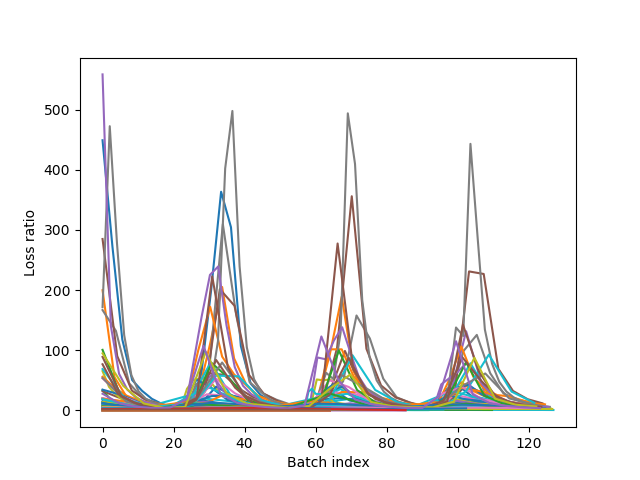
\includegraphics[scale=0.7]{experiments/epochs/25-epochs.png}
	\end{center}
	\caption{The ratio between the highest error event in the batch and the average error in the batch. Every line represents a user. Amount of batches normalized against the user with the most batches and cut off at 20 batches. Using 25 epochs.~\label{fig:25-epochs}}
\end{figure}


\begin{figure}
	\begin{center}
		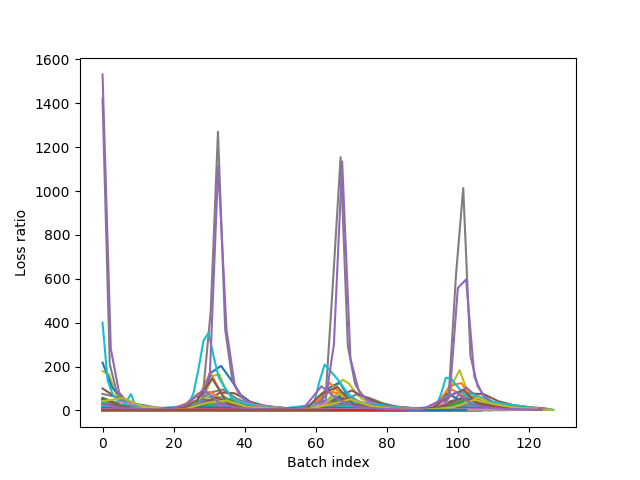
\includegraphics[scale=0.7]{experiments/epochs/15-epochs}
	\end{center}
	\caption{The ratio between the highest error event in the batch and the average error in the batch. Every line represents a user. Amount of batches normalized against the user with the most batches and cut off at 20 batches. Using 15 epochs.~\label{fig:15-epochs}}
\end{figure}


\begin{figure}
	\begin{center}
		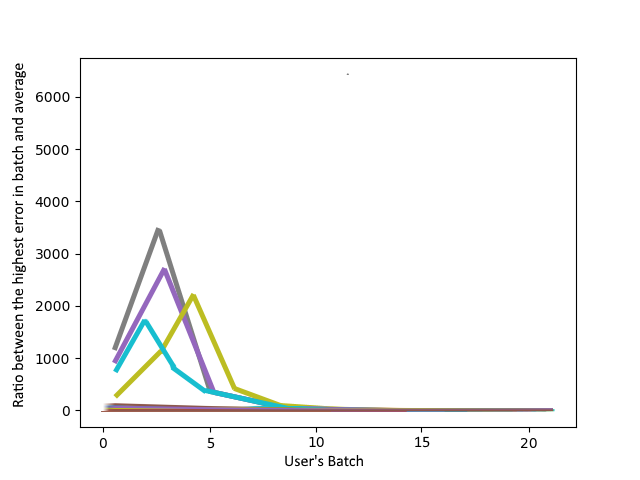
\includegraphics[scale=0.7]{experiments/epochs/8-epochs}
	\end{center}
	\caption{The ratio between the highest error event in the batch and the average error in the batch. Every line represents a user. Amount of batches normalized against the user with the most batches and cut off at 20 batches. Using 8 epochs.~\label{fig:8-epochs}}
\end{figure}

\section{Shared weights}
The possibility of using one neural network for all users was explored. However, this introduced some problems. One of these is that the total number of actions for all users was not the same. This leads to the system weighing the actions of high-volume users heavier than those of low-volume users, leading to an unfair representation of the \enquote{average} user's behavior. Another problem was that performance was significantly worse. Parallelization can not be applied as the single network has to be kept in memory for the entire process. The network also gravitates towards learning the behavior of \enquote{average} users. It will try to find a middle ground in the behavior of different types of users (sysadmins vs users that rarely log in), never really learning a single user's behavior well enough to find slight deviations. It will then accept users such as sysadmins having a high error value as normal, which could be very dangerous if such an account gets compromised.

\section{GRU cell}
Usage of a different RNN cell has also been explored. One of these different RNN cells is the GRU cell, introduced in~\cite{cho2014learning}. The differences between an architecture using a LSTM cells and an architecture using GRU cells are slight. As~\cite{chung2014empirical} showed, the performance of GRU cells and LSTM cells are very similar when it came to the area of polyphonic music modeling and speech signal modeling. As such, it is likely that their performance on the area of cyber-security is also similar. 

In order to get an idea of how much the error between the predicted feature vector and the actual feature vector deviates from that user's mean error, a function has been created with which this can be calculated. When replacing 1.5 with \(y\) in equation~\ref{eq:iqr_max}, with \(x\) being the mean squared error (function~\ref{eq:mse}) between the predicted feature vector and the actual feature vector, solving for \(y\) gives the following function:

\begin{equation} \label{eq:y}
y = (x - Q3) / IQR
\end{equation}

This \(y\) value is plotted for the different architectures (GRU and LSTM with the parameters described above), which can be seen in Figure~\ref{fig:gru_vs_lstm}. This figure shows the GRU and LSTM deviations being fairly close. In the lowest group (from 0 to 18) the LSTM seems to be consistently higher than the GRU, however, at this scale the difference isn't that big. If you draw lines through these points, the lines run parallel (when viewing the plot non-logarithmically), showing that the architectures find similar anomalies. In later groups, the GRU has consistently higher \(y\) scores than the LSTM. This can point to it flagging actual anomalies as more anomalous (pointing to it being better at recognizing them), or it labeling non-anomalous actions as more likely to be anomalies. Because the data set is unlabeled there is unfortunately no way to find out. Figure~\ref{fig:gru_rnn_losses} again shows that the architecture using LSTMs has a higher error value for most batches, also peaking higher. The LSTM architecture also flagged 0.7\% more events as anomalies. Again conclusions can not be drawn regarding which result is more effective but it can be seen that they do differ somewhat.

\begin{figure}
	\begin{center}
		\includegraphics[scale=0.8]{experiments/cell/deviations/gru_vs_lstm}
	\end{center}
	\caption{The deviations \(y\) (function~\ref{eq:y}). Where the IQR is being calculated over the training set and \(x\) is the mean squared error between a predicted feature vector and the actual feature vector. Combining the last 5 actions for each user, over 0.1\% of all users (sorted). Comparing GRU and LSTM.~\label{fig:gru_vs_lstm}}
\end{figure}

\begin{figure}
	\begin{center}
		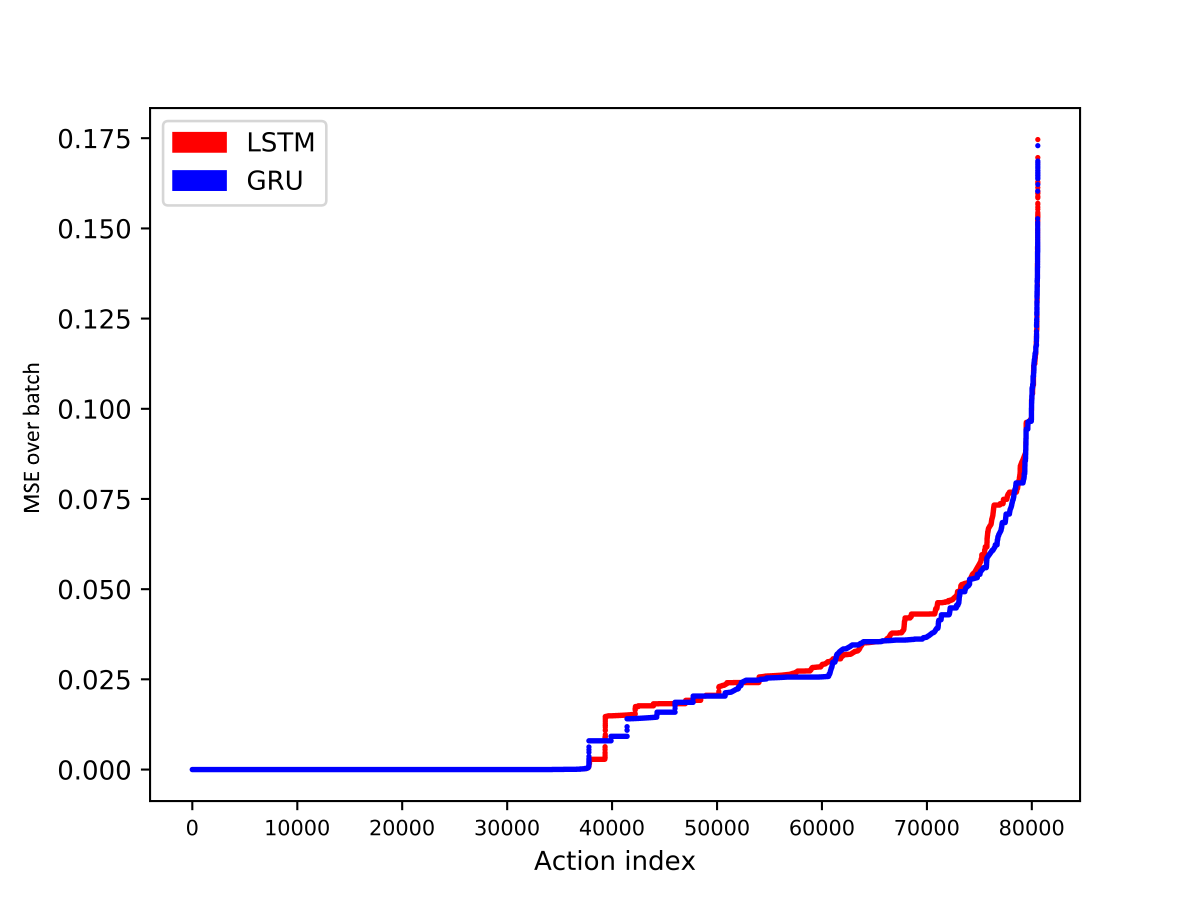
\includegraphics[scale=6.0]{experiments/cell/losses/comparison}
	\end{center}
	\caption{The error of all users' actions combined, calculated using the mse (sorted).~\label{fig:gru_rnn_losses}}
\end{figure}

\section{RNN cell}
Using standard RNN cells instead of LSTM cells showed a significant difference. The parameters to the RNN were the same as those to the LSTM network. The RNN cells seem to have significantly higher errors in the middle group (18 to 35), while having significantly lower errors in the last group, as can be seen in Figure~\ref{fig:rnn_vs_lstm}. The RNN cells also flagged less events as anomalous, flagging 21\% less as such. Once again no clear conclusion can be drawn as to which one is more effective, however, LSTMs have been shown to be superior to regular RNNs in many fields, suggesting that this may also be a case of the LSTM cells outperforming the RNN cells at flagging anomalies.

\begin{figure}
	\begin{center}
		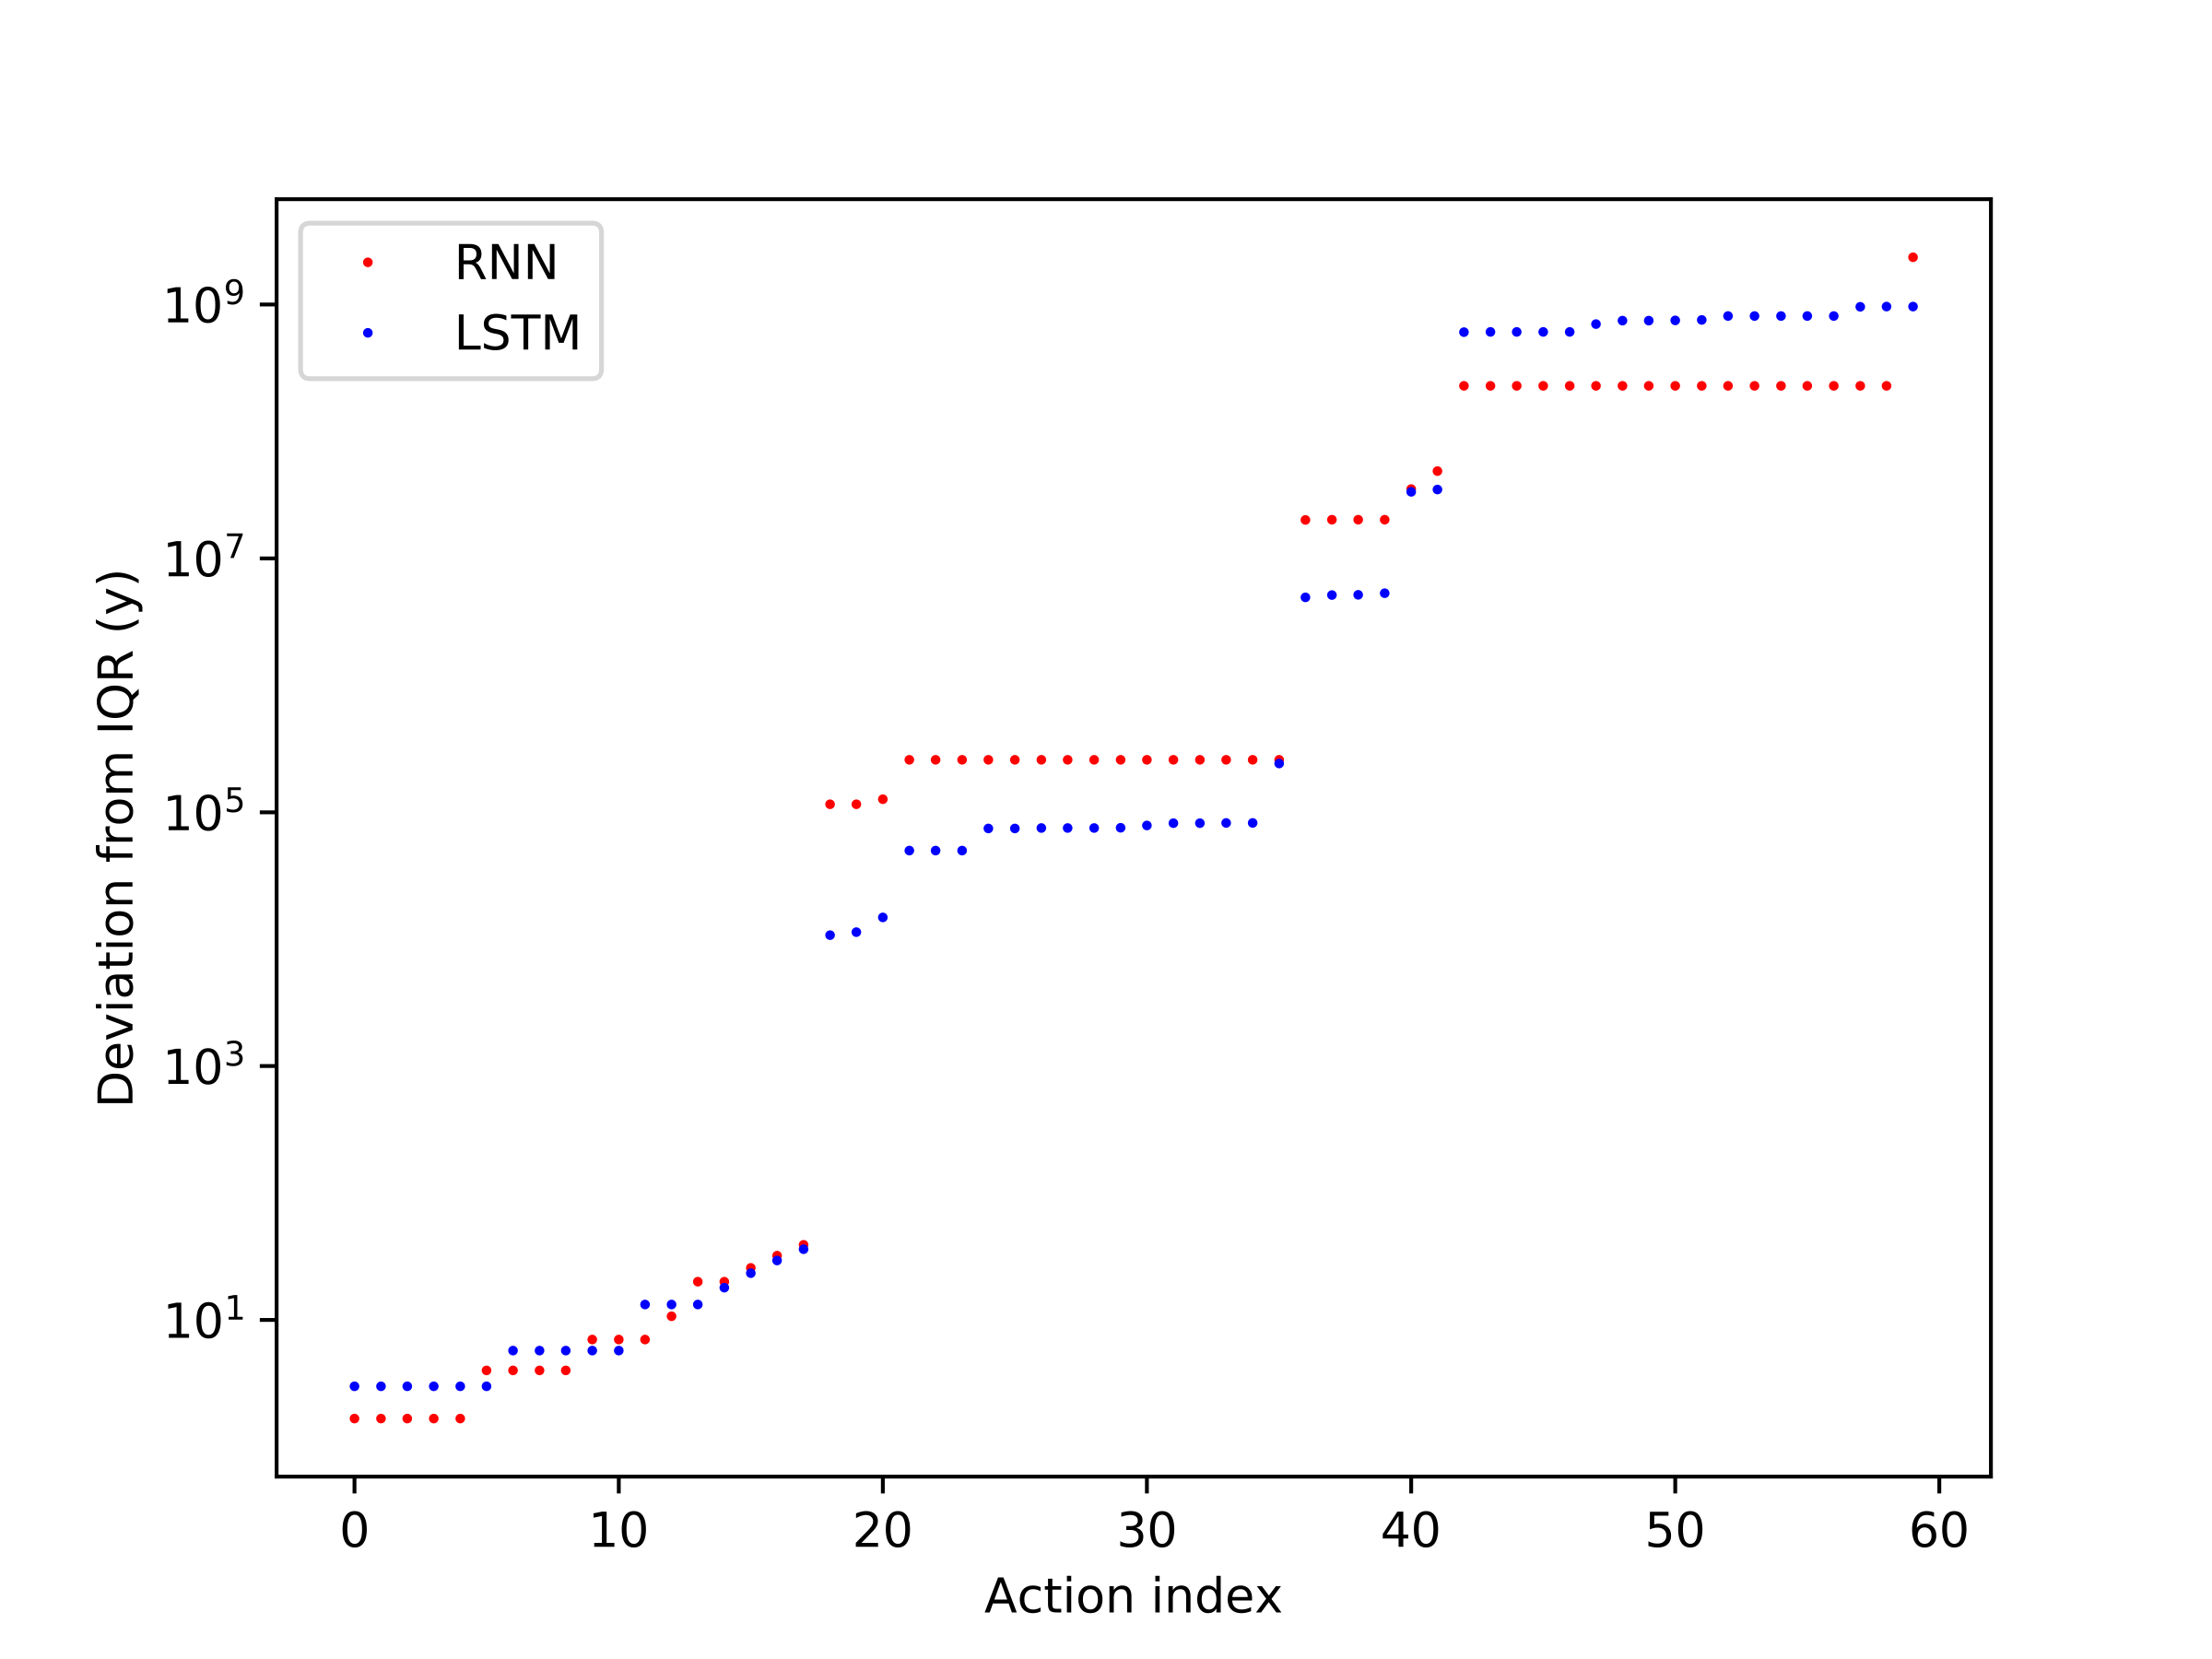
\includegraphics[scale=0.8]{experiments/cell/deviations/rnn_vs_lstm}
	\end{center}
	\caption{The deviations \(y\) (function~\ref{eq:y}). Where the IQR is being calculated over the training set and \(x\) is the mean squared error between a predicted feature vector and the actual feature vector. Combining the last 5 actions for each user, over 0.1\% of all users (sorted). Comparing plain RNN and LSTM.~\label{fig:rnn_vs_lstm}}
\end{figure}
